%%% LaTeX Template: Article/Thesis/etc. with colored headings and special fonts
%%%
%%% Source: http://www.howtotex.com/
%%% Feel free to distribute this template, but please keep the referral to http://www.howtotex.com/ here.
%%% February 2011
%%%
%%% Last updated September 2021 by CDM

%%%%%%%%%%%%%%%%%%%%%%%%%%%%%%%%%%%%%%%%%%
%%%%%%%%%%%%%% Preamble %%%%%%%%%%%%%%%%%%
%%%%%%%%%%%%%%%%%%%%%%%%%%%%%%%%%%%%%%%%%%
\documentclass{article}
\usepackage[margin=1.0in]{geometry}
\usepackage[T1]{fontenc}
\usepackage[bitstream-charter]{mathdesign}
\usepackage[latin1]{inputenc}					
\usepackage{amsmath}						
\usepackage{xcolor}
\usepackage{cite}
\usepackage{hyphenat}
\usepackage{graphicx}
\usepackage{float}
\usepackage{subfigure}
\usepackage{sectsty}
\usepackage[compact]{titlesec} 
\usepackage[tablegrid]{vhistory}
\allsectionsfont{\color{accentcolor}\scshape\selectfont}

%%%%%%%%%%%%%%%%%%%%%%%%%%%%%%%%%%%%%%%%%%
%%%%%%%%%%% Definitions %%%%%%%%%%%%%%%%%%
%%%%%%%%%%%%%%%%%%%%%%%%%%%%%%%%%%%%%%%%%%
\definecolor{accentcolor}{rgb}{0.0,0.0,0.5} 
\newcommand{\teamname}{Top Drone: Mavericks}
\newcommand{\productname}{Raytheon Drone Project}
\newcommand{\coursename}{CSE 4316: Senior Design I}
\newcommand{\semester}{Fall 2022}
\newcommand{\docname}{Project Charter}
\newcommand{\department}{Department of Computer Science \& Engineering}
\newcommand{\university}{The University of Texas at Arlington}
\newcommand{\authors}
{
Jaedyn Brown
\\ Robert Carr
\\ Javier Lopez
\\ Ja'lun Morris
\\ Pearl Iyayi
}

%%%%%%%%%%%%%%%%%%%%%%%%%%%%%%%%%%%%%%%%%%
%%%%%%%% Headers and Footers %%%%%%%%%%%%%
%%%%%%%%%%%%%%%%%%%%%%%%%%%%%%%%%%%%%%%%%%
\usepackage{fancyhdr}
	\pagestyle{fancy}						% Enabling the custom headers/footers
\usepackage{lastpage}	
	% Header (empty)
	\lhead{}
	\chead{}
	\rhead{}
	% Footer
	\lfoot{\footnotesize \teamname \ - \semester}
	\cfoot{}
	\rfoot{\footnotesize page \thepage\ of \pageref{LastPage}}	% "Page 1 of 2"
	\renewcommand{\headrulewidth}{0.0pt}
	\renewcommand{\footrulewidth}{0.4pt}

%%%%%%% Change the abstract environment %%%%%%%
\usepackage[runin]{abstract}			% runin option for a run-in title
\abslabeldelim{\quad}	
\setlength{\abstitleskip}{-10pt}
\renewcommand{\abstractname}{}
\renewcommand{\abstracttextfont}{\color{accentcolor} \small \slshape}	% slanted text


%%%%%%%%%%%%%%%%%%%%%%%%%%%%%%%%%%%%%%%%%%
%%%%%%%%%% Start of the Document %%%%%%%%%
%%%%%%%%%%%%%%%%%%%%%%%%%%%%%%%%%%%%%%%%%%
\begin{document}

%%%%%%%%%%%%%% Cover sheet %%%%%%%%%%%%%%%
{\centering \huge \color{accentcolor} \sc \textbf{\department \\ \university} \par}
\vspace{1 in}
{\centering \huge \color{accentcolor} \sc \textbf{\docname \\ \coursename \\ \semester} \par}
\vspace{0.5 in}
\begin{figure}[h!]
	\centering
   	
\includegraphics[width=0.60\textwidth]{images/Final_Logo.png}
\end{figure}
\vspace{0.5 in}
{\centering \huge \color{accentcolor} \sc \textbf{\teamname \\ \productname} \par}
\vspace{0.5 in}
{\centering \large \sc \textbf{\authors} \par}
\newpage

%%%%%%%%%%%% Revision History %%%%%%%%%%%%
\begin{versionhistory}
  	\vhEntry{0.1}{09.12.2022}{RC, JB, JL, JM, PI}{document creation}
  	\vhEntry{0.2}{10.03.2022}{RC, JB, JL, JM, PI}{complete draft}
\end{versionhistory}
\newpage

%%%%%%%%%%%% Table of contents %%%%%%%%%%%%
\tableofcontents
\newpage

%%%%%% List of figures and tables (optional) %%%%%%
\listoffigures
%\listoftables
\newpage
\setcounter{table}{0}

%%%%%% Executive summary sections %%%%%%

% 1 PROBLEM STATEMENT
\section{Problem Statement}
This project is being undertaken in response to the growing demand for Unmanned Aircraft Systems (UAS). With drone technology, there is an increasing flexibility in the tasks that can be accomplished. The scenario that is presented is to be able to identify friendly ground vehicles and disarm hostile vehicles. In this use case, having a UAS that can fly autonomously and identify enemy vehicles could be used in various ways.

% 2 METHODOLOGY
\section{Methodology}
% This file contains the text portion of the Methodology portion of the project charter

% 2 METHODOLOGY
By researching and developing software that allows for the full autonomy of airborne drones, the student CSE team will address the rapidly growing demand for autonomous aircraft systems. Under the mentorship of Raytheon, the team will develop an autonomous ground vehicle and drone through coordination with undergraduate students studying Electrical Engineering (EE) and Mechanical and Aerospace Engineering (MAE). By utilizing ArUco markers, the drone's camera will enable it to identify ground targets during flight to distinguish friends from enemies. Upon detecting hostile ground vehicles within a 50-yard-by-50-yard area, the drone will fire a laser at the moving ground vehicle to indicate if the drone has successfully engaged and hit the target.


% 3 VALUE PROPOSITION
\section{Value Proposition}
The project is sponsored by Raytheon Technologies, an American multinational aerospace and defense company.  In its role as a world leader in aerospace and defense, Raytheon understands the importance of investigating and developing unmanned systems. Raytheon will get to work with and monitor student teams and guide them as they develop unmanned air and ground vehicles through a two-semester-long project. Using this mechanism, Raytheon can identify top graduates, promote corporate recruitment, and explore the latest technology trends.

% 4 DEVELOPMENT MILESTONES
\section{Development Milestones}
% This file contains the text portion of the Development Milestones portion of the project charter

% 4 DEVELOPMENT MILESTONES
\begin{itemize}
    \item Requirements Review - September 2022
    \item Project Planning - September 2022
    \item Project Charter first draft - October 2022
    \item System Requirements Specification - September 2022
    \item Architectural Design Specification - September 2022
    \item Project Proposal \& Presentation - October 2022
    \item Mid-Year Report - December 2022
    \item Prototype Creation - December 2022
    \item Prototype Demonstration - December 2022
    \item Targeting Showcase 1 - January 2023
    \item Targeting Showcase 2 - February 2023
    \item Targeting Showcase 3 - March 2023
    \item Targeting Showcase 4 - April 2023
    \item CoE Innovation Day poster Presentation - April 2023
    \item Final Project Presentation - May 2023
\end{itemize}


\newpage

%%%%%%% Remaining Project Charter Sections %%%%%%%

% 5 BACKGROUND
\section{Background}
% This file contains the text portion of the Background portion of the project charter


% 5 BACKGROUND
As of 2025, unmanned aircraft systems are expected to create more than 100,000 jobs, according to a study by the Association for Unmanned Vehicle Systems International (AUVSI) (credit here: Robert found this, I will add it later). As warfare becomes more dangerous and technologies advance, militaries are looking for ways to minimize their losses. Rather than putting their troops in harm's way, military leaders want autonomous vehicles that can take down hostile targets. It is Raytheon's goal to support student research and innovation in autonomous vehicle design by sponsoring them in this showcase competition. As a result, Raytheon is able to scout and recruit top graduates from universities participating in the showcase. Students will have to research and develop algorithms that use computer vision. In addition to developing algorithms that use computer vision, students will gain industry insight while collaborating across multiple teams and coordinating for a long project that requires extensive documentation and coordination.

% A new paragraph with tab just needs an empty line
In addition to providing Raytheon with technology for national defense purposes, the AUVSI report estimates that the integration of these systems with the National Airspace System (NAS) between 2015 and 2025 will generate more than 80 billion dollars. This is due to the many applications for UASs in the following areas: wildfire mapping, agriculture, disaster management, law enforcement, cinema, environmental monitoring, and freight transport (cite: Robert). There has been no prior relationship between the software development team and Raytheon, but this is expected to develop in the future.


% 6 RELATED WORK
\section{Related Work}
% This file contains the text portion of the Related Work portion of the project charter

% 6 RELATED WORK


% 7 SYSTEM OVERVIEW
\section{System Overview}
% This file contains the text portion of the System Overview portion of the project charter

% 7 SYSTEM OVERVIEW
It is assumed that the drone will be equipped with a single-board computer in the diagram below. Using a single-board computer, the drone would be able to process the tasks it is required to carry out for each showcase by executing them through the single-board computer. It is still unknown whether the computation part of the project will be allowed to be performed wirelessly (i.e. without the need for an onboard computer to control the drone) by the team. Once a decision has been made, a new version of this document will be prepared.

It is expected that a flight controller will be mounted on the drone in order to control the motors' speeds, therefore allowing horizontal and vertical movement in the drone to take place. It will be necessary to run Mission Planner on a computer (either onboard or via a wireless connection) in order for it to function. With the help of Mission Planner, drone movements can be mapped for the drone so it can be controlled as needed. With Mission Planner, autonomous vehicles can communicate with a ground station via an interface which can be accessed from most Windows operating systems. As a result of using Mission Planner, the team will have the option of creating their own autonomous flight paths. Further, the computer will run a program that has the capability of identifying ArUco markers as well as functioning as a link between the computer and the flight controller.

For aiming at the ace combat sensors that are located on all hostile ground vehicles, there needs to be a laser attached close to the camera to increase accuracy. There are two choices available to the camera once it detects an ArUco marker. The camera can either turn and aim at the enemy vehicle or move to a position where the drone could use its laser to shoot moving ground vehicles.

There will be a dedicated flight controller that will be connected to GPS and RTK systems. It is expected that the drone motors will be connected to electronic speed controllers, which will in turn be connected to the dedicated flight controller.

To power all of the components of the drone while it is in flight, the drone will need to be equipped with a battery. There is no doubt that batteries can add a lot of weight to a drone, so this is also something that should be considered when deciding which batteries to use. Battery size and location should also be considered in order to ensure that the camera or laser is not interfered with or blocked by the battery in any way.

\begin{figure}[h!]
    \centering
    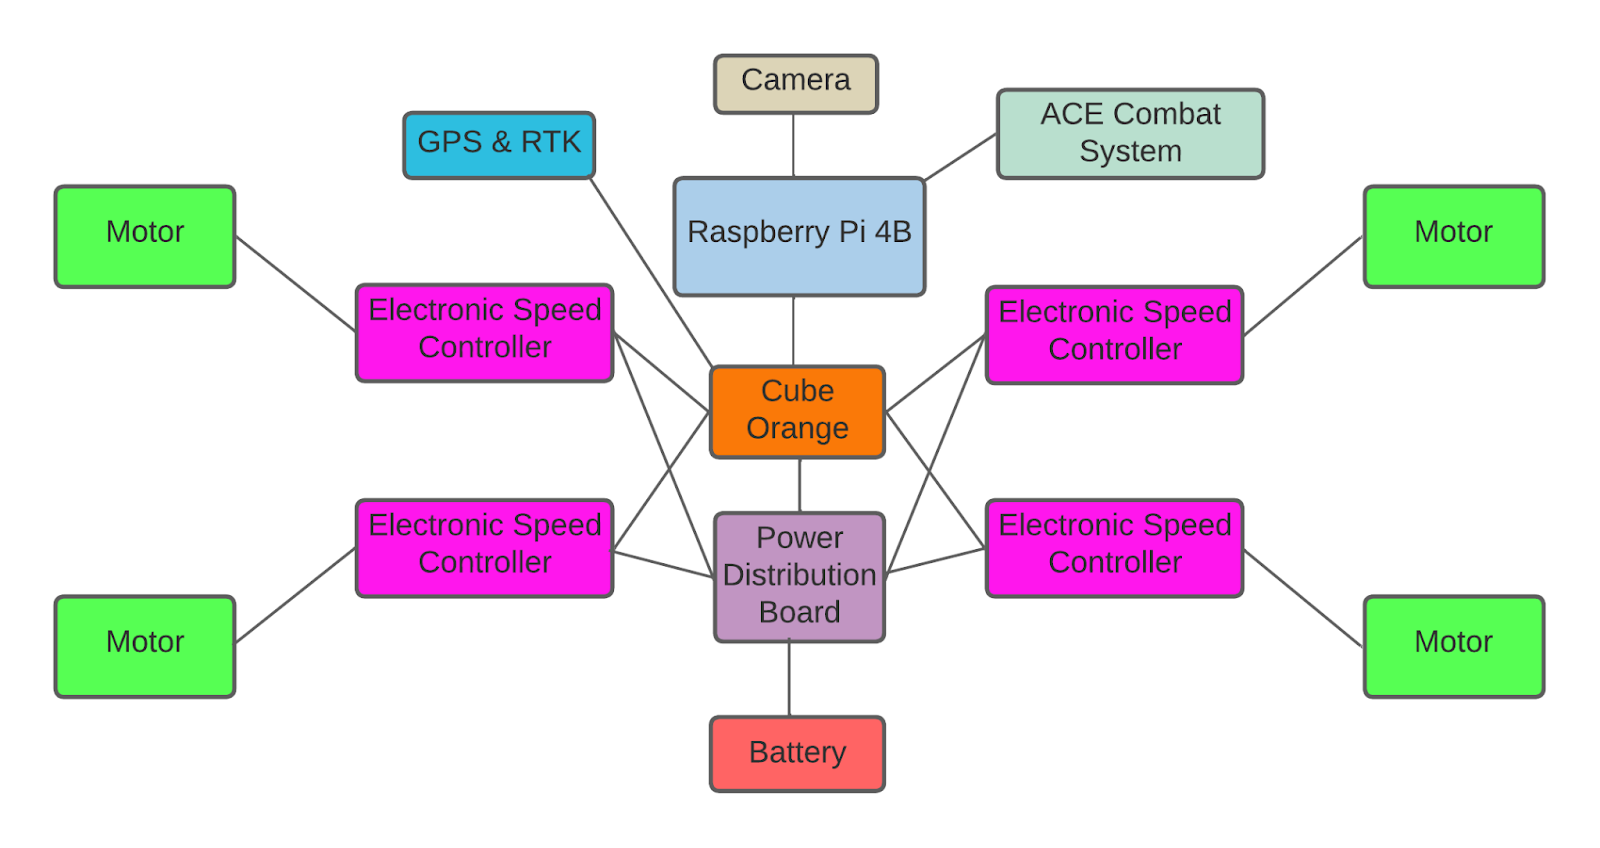
\includegraphics[width=1\textwidth]{images/system_overview.png}
    \caption{Diagram of the System Overview}
\end{figure}


% 8 ROLES & RESPONSIBILITIES
\section{Roles \& Responsibilities}
% This file contains the text portion of the Roles & Responsibilities portion of the project charter

% 8 ROLES & RESPONSIBILITIES
Raytheon's stakeholders include the following two members:
\begin{itemize}
    \item Gretchen Mock (RIS Senior Leadership) - Raytheon Mentor \& Point of Contact
    \item Jesse Lee (Competition Council) - UT Student Mentor
\end{itemize}
For this project, the CSE team consists of the following five students:
\begin{itemize}
    \item Javier - Student Team Lead \& Point of Contact
    \item Jaedyn Brown - Student Team Member \& SCRUM Master
    \item Robert Carr - Student Team Member \& FAA Certified UAV Pilot
    \item Ja'Lun Morris - Student Team Member
    \item Pearl Iyayi - Student Team Member
\end{itemize}
Currently, it is unclear what specific roles each member will be assigned, such as computer vision or autonomous flight. The current team lead and point of contact is Javier Lopez, who manages the student team and represents the team to McMurrough, the Raytheon mentors, and the student leader of the entire project. As well as being a student team member, Robert Carr will get his FAA UAV pilot certification. Prior to demonstrations, Robert will need to pass the relevant examinations and ensure that the drone is safe to fly within regulations. Jaedyn Brown holds the position of SCRUM master and is therefore primarily in charge of laying out the sprint backlog for each sprint, and giving time estimates for how long each of those tasks should take. The position of SCRUM master will be maintained throughout the duration of the project as Jaedyn's role.


% 9 COST PROPOSAL
\section{Cost Proposal}
% This file contains the text portion of the Cost Proposal portion of the project charter

% 9.1 PRELIMINARY BUDGET
\subsection{Preliminary Budget}
In addition to the parts below, FAA Pilot Certifications will be required. Two certifications (\$175 each) will be acquired for a total of \$350.

% 9.2 CURRENT & PENDING SUPPORT
\subsection{Current \& Pending Support}
\begin{itemize}
  \item \$5,000 will be provided by Raytheon Technologies
  \item \$800 will be provided by the University of Texas at Arlington
\end{itemize}

% 10 FACILITIES & EQUIPMENT
\section{Facilities \& Equipment}
% This file contains the text portion of the Facilities & Equipment portion of the project charter

\begin{itemize}
  \item UTA Maverick Stadium
  \item Senior Design Lab located in ERB 335
  \item 3D printer
  \item Makerspace
\end{itemize}

% 11 ASSUMPTIONS
\section{Assumptions}
% This file contains the text portion of the Assumptions portion of the project charter
%   The following may be helpful for encoding errors: https://www.charset.org/utf8-to-latin-converter


\begin{itemize}
  \item Drone flight tests can be conducted on campus.
  \item Dedicated campus lab spaces will be made available for the software development team to meet and develop software.
  \item Hardware development of the unmanned ground vehicle is primarily the responsibility of the EE and MAE teams.
  \item It is expected that the EE and MAE teams will have a working ground vehicle available to the software development team when it is needed.
\end{itemize}

% 12 CONSTRAINTS
\section{Constraints}
% This file contains the text portion of the Constraints portion of the project charter

% 12 CONSTRAINTS
\begin{itemize}
  \item The project must be completed by April.
  \item For each challenge demonstration, the project must be in a working state.
  \item Raytheon provides \$5,000 for team-wide development costs. In the event that we go over this, we will need to look for outside funding.
  \item The project demo deadline must be met with a demonstrable portion of the project.
\end{itemize}


% 13 RISKS
\section{Risks}
% This file contains the text portion of the Risks portion of the project charter

% 13 RISKS
% For tables in LaTeX, see: https://www.overleaf.com/learn/latex/Tables
\begin{table}[h]
    \resizebox{\textwidth}{!}{
        \begin{tabular}{|l|l|l|l|}
            \hline
            \textbf{Risk description} & \textbf{Probability} & \textbf{Loss (days)} & \textbf{Exposure (days)} \\ \hline
            Software team experiencing delays caused by other teams & 0.5 & 30 & 15 \\ \hline
            Drone crash during testing & 0.8 & 14 & 11.2 \\ \hline
            Part availability may delay shipping & 0.6 & 14 & 8.4 \\ \hline
            Replacement of faulty or damaged drone hardware & 0.4 & 12 & 4.8 \\ \hline
            Outsiders messing with and breaking the drone & 0.05 & 14 & 0.7 \\ \hline
        \end{tabular}}
    \caption{Overview of highest exposure project risks}
\end{table}


% 14 DOCUMENTATION & REPORTING
\section{Documentation \& Reporting}
% This file contains the text portion of the Documentation & Reporting portion of the project charter - Section 14

%%%%%%%%%%%%%%%%%%%%%%%%%%%%%%%%%%%%%%%%%%%%%%
%%%%%%% 14.1 DOCUMENTATION & REPORTING %%%%%%%
%%%%%%%%%%%%%%%%%%%%%%%%%%%%%%%%%%%%%%%%%%%%%%
% 14.1 MAJOR DOCUMENTATION DELIVERABLES
\subsection{Major Documentation Deliverables}

% 14.1.1 PROJECT CHARTER
\subsubsection{Project Charter}
The initial version of the Project Charter will be uploaded on October 3nd 2022. The final version of the Project charter will be uploaded on April 30th 2023. There is a possibility that the charter will be updated sprint to sprint as more information is received. Sections such as 14.2, 14.2.1, 14.2.5, etc, are most likely to be updated.

% 14.1.2 SYSTEM REQUIREMENTS SPECIFICATION
\subsubsection{Systems Requirements Specification}
The initial version of the SRS document will describe the features and behaviors of the Drone and the software we expect to utilize within the project. The initial version of the SRS document will be submitted on October 24, 2022. The final version of the SRS document will be submitted on April 30th, 2023 when the final version of the project charter will be submitted. Should changes occur after the initial version of the SRS document is submitted, we will update the appropriate document/s to reflect those changes.

% 14.1.3 ARCHITECTURAL DESIGN SPECIFICATION
\subsubsection{Architectural Design Specification}
November 14th, 2022 will be the deadline for the initial Architectural Design Specification (ADS). The final deadline for the ADS will be April 30th, 2022. Each team member can edit the ADS at any time, and all changes will be reflected for everyone on a shared Google Doc. In the process of developing the project, we will continue to update this shared document as needed.

% 14.1.4 DETAILED DESIGN SPECIFICATION
\subsubsection{Detailed Design Specification}
The initial version of the Detailed Design Specification (DDS) will reflect the state of hardware and software components at that time. If any changes are made to the hardware or software being utilized in the project after the initial version is submitted, then our team will update the DDS to reflect those changes. The initial version of the Detailed Design Specification will be submitted February 26th, 2023. The final version of the Detailed Design Specification will be submitted April 30th, 2023.

%%%%%%%%%%%%%%%%%%%%%%%%%%%%%%%%%%%%%%%%%%%%%%
%%%%%%%%% 14.2 RECURRING SPRINT ITEMS %%%%%%%%
%%%%%%%%%%%%%%%%%%%%%%%%%%%%%%%%%%%%%%%%%%%%%%
\subsection{Recurring Sprint Items}

% 14.2.1 PRODUCT BACKLOG
\subsubsection{Product Backlog}
As soon as the SRS is created, a backlog item will be created for each requirement. These items will be prioritized by necessity to get a test drone built, while also having working software. The handling of our team's backlog will be done by the Scrum Master. The team's backlog will be issued through a shared Google Sheet.

% 14.2.2 SPRINT PLANNING
\subsubsection{Sprint Planning}
There will be eight sprints throughout the duration of this project. Each of them would be planned taking into account lessons learned from previous sprints. The following methods will also be implemented:
\begin{itemize}
  \item Planning a sprint meeting after examining the team's availability
  \item Go over backlog and assigning ownership of tasks to team members
  \item Confirm new issues, impacts, and dependencies
  \item Reach a group consensus on time estimations
\end{itemize}

% 14.2.3 SPRINT GOAL
\subsubsection{Sprint Goal}
The sprint goal will be determined by the team during a meeting before the start of the sprint. The best way to keep the project stakeholders involved is by giving a report on our sprint goal to our sponsor on the first Friday of every sprint.

% 14.2.4 SPRINT BACKLOG
\subsubsection{Sprint Backlog}
The SCRUM master will be primarily in charge of managing which items are placed in the sprint backlog, and how much time is estimated for each of those tasks. An excel spreadsheet will be used to maintain our sprint backlog, update time estimates, and display a burndown chart.

% 14.2.5 TASK BREAKDOWN
\subsubsection{Task Breakdown}
Individual tasks will be first assigned by members who volunteer for that task. Time spent on tasks will be logged by each individual within the team on our Excel spreadsheet.

% 14.2.6 SPRINT BURN DOWN CHARTS
\subsubsection{Sprint Burn Down Charts}
When each team member logs their hours worked for each task in the Excel spreadsheet, there will be a Burn Down chart that gets updated automatically. The sprint spreadsheet will include specific sprint backlogs in which the general tasks for that sprint are divided into smaller parts. This will indicate which team member(s) worked on each subtask. The subtasks are not recorded per hour, yet. The total number of hours expended by each team member is included in a table for every sprint backlog.

\begin{figure}[h!]
    \centering
    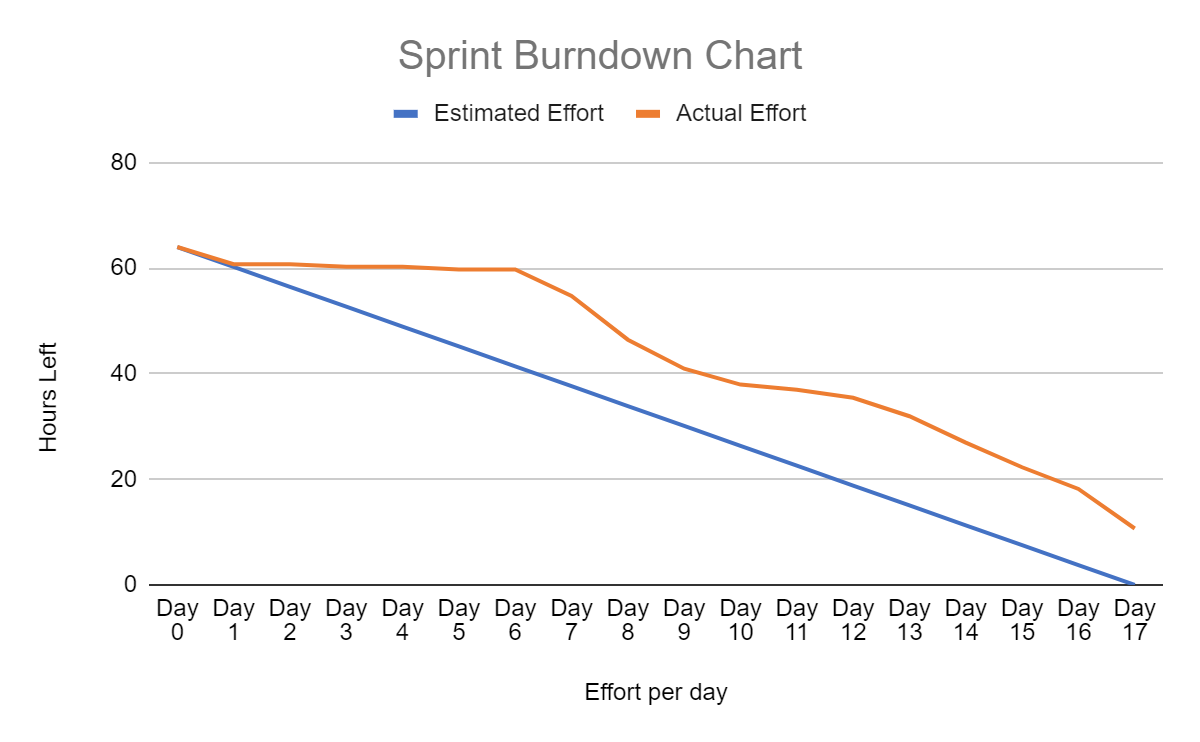
\includegraphics[width=1\textwidth]{images/burndown_example.png}
    \caption{Example sprint burn down chart}
\end{figure}

% 14.2.7 SPRINT RETROSPECTIVE
\subsubsection{Sprint Retrospective}
Following each sprint, the team will hold a retrospective meeting to discuss what went well and what could be improved. We will assign team tasks to each team member based on the sprint goals. Assigning tasks will keep team members accountable. Each task will be due at the end of each sprint.

% 14.2.8 INDIVIDUAL STATUS REPORTS
\subsubsection{Individual Status Reports}
Every week, there will be a Discord meeting to give a status report. Detailed information regarding a team member's goals, issues, and progress will be included in the team member's status reports.

% 14.2.9 ENGINEERING NOTEBOOKS
\subsubsection{Engineering Notebooks}
Software development team members are expected to update their engineering notebooks at the end of each sprint in order to hold each other accountable for their work. It is essential that each team member is able to communicate effectively regarding their engineering notebooks in order to hold one another accountable. A mid-sprint meeting can be used to discuss the targeted number of pages for the current sprint. To ensure quality control, the SCRUM master must sign off as a witness for each engineering notebook page.

%%%%%%%%%%%%%%%%%%%%%%%%%%%%%%%%%%%%%%%
%%%%%%% 14.3 CLOSEOUT MATERIALS %%%%%%% 
%%%%%%%%%%%%%%%%%%%%%%%%%%%%%%%%%%%%%%%
\subsection{Closeout Materials}

% 14.3.1 SYSTEM PROTOTYPE
\subsubsection{System Prototype}
In the final system prototype the drone will contain features that have been discussed in previous sections. To reiterate, the final system prototype will include the following: GPS and RTK, camera for IR blasting and QR code detection, a cube orange flight controller, and software that configures autonomous flight. There will be a Prototype Acceptance Test with the customer, they expect to see a prototype by the end of the fall 2022 semester. There will be off-site testing in the Maverick stadium as it is intended to be an outdoor competition if there are favorable weather conditions.

% 14.3.2 PROJECT POSTER
\subsubsection{Project Poster}
In addition to an architectural diagram, the poster will also explain Python use cases and describe the components of the drone.

% 14.3.3 WEB PAGE
%\subsubsection{Web Page}

% 14.3.4 DEMO VIDEO
\subsubsection{Demo Video}
As certain parts of the project become demonstrable, demo videos will be provided. Demo videos will demonstrate key aspects of the project and how they behave and respond in real-world environments. Videos will vary in length depending on what is being demonstrated.

% 14.3.5 SOURCE CODE
\subsubsection{Source Code}
Version control and source code maintenance will be handled by the team using Git and GitHub. The source code will not be accessible to the public at any time during the project's lifecycle. It will however, be available to Raytheon and the entire student team. A zipped folder from the GitHub repository could be provided at any time to enable users to view the source code at any time. License information, if included, will appear at the top level of the folder structure to make it easy to locate.

% 14.3.6 SOURCE CODE DOCUMENTATION
\subsubsection{Source Code Documentation}
Our team does not currently have any plans for what tool may be utilized in order to assist in documentation. These tools will be explored in deeper detail and when a decision is made, the Project Charter will have documentation produced in LaTeX.

% 14.3.7 HARDWARE SCHEMATICS
\subsubsection{Hardware Schematics}
The hardware schematics will be updated when the parts that will be used to assemble the drone for the CSE test run are confirmed. Right now its is known that there will be soldering needed to make some electrical connections.

% 14.3.8 CAD FILES
%\subsubsection{CAD Files}

% 14.3.9 INSTALLATION SCRIPTS
%\subsubsection{Installation Scripts}

% 14.3.10 USER MANUAL
\subsubsection{User Manual}
This project's user manual will be available at a later date. A setup video may be included in the user manual explaining how the hardware is configured and how to run the code. In the case a video is included, the visual instructions will show how to run the project in a simple and straightforward manner.


\newpage

%%% References
% If I remove the below line, the bib error goes away, will leave it for now
%   See: https://tex.stackexchange.com/questions/631323/error-message-from-bibtex-illegal-another-bibstyle-command
%\bibliographystyle{plain}
\bibliographystyle{reference/IEEEtran_custom}
\bibliography{reference/refs}{}

\end{document}
